\section{需求分析}
   本程序将利用先序遍历所得序列,建立一棵可以唯一确定的二叉树。
   使用\#标志一个输入的结束。支持输入多个数据。


   程序具有判定和输出所建成的二叉树的功能。
   程序会判定输入是否合法,比如a***可以判定为一个不合法的输入。


   此时程序会输出 Input Error


   当二叉树建成时,程序会使用广义表的方式输出二叉树。
   例如样例中的二叉树可以输出为


   a(b(c, d), e)
   
\section{概要设计}
   首先我们要定义一个使用二叉链表表示的结构体。
   \begin{enumerate}
      \item TreeNode* lch  储存左子树
      \item TreeNode* rch  储存右子树
      \item char  data  储存数据
   \end{enumerate}


   再定义一个解决问题的类
   \begin{enumerate}
      \item printTree() 输出二叉树的广义表行事
      \item inputTree() 输入一个字符串并将该字符串转化为二叉树
      \item buildTree() 传入指针,递归建树
   \end{enumerate}

\newpage

\section{详细设计}

\begin{algorithm}[htb] 
   \caption{ inputTree } 
   \label{alg:Framwork} 
   \begin{algorithmic}[1]
      \Function {inputTree}{void}
         \State 读入字符串,并保存在str中
         \State 初始化根节点为root
         \If {buildTree(root, str, 1) == str的长度}
            \State printTree(root)
         \Else
            \State 打印Input Error
         \EndIf
      \EndFunction
   \end{algorithmic} 
\end{algorithm}

\begin{algorithm}[htb] 
   \caption{ buildTree } 
   \label{alg:Framwork} 
   \begin{algorithmic}[1]
      
      \Function {buildTree}{root, str, n}
      \If {str[n]是*}
         \State \Return n
      \Else
         \State root结点的数据设为str[n]
         \State 初始化lch
         \State n = buildTree(lch, str, n + 1)
         \State 初始化rch
         \State n = buildTree(rch, str, n + !)
         \State \Return n
      \EndIf
   \EndFunction

   \end{algorithmic} 
\end{algorithm}

\newpage

\begin{algorithm}[htb] 
   \caption{ printTree } 
   \label{alg:Framwork} 
   \begin{algorithmic}[1]
      \Function {printTree}{root}
         \If{root 为空}
            \State \Return
         \Else
            \State 输出root数据
            \If{root存在子树}
               \State 输出(
                  \State printTree(lch)
                  \State 输出,
                  \State printTree(rch)
               \State 输出)
            \EndIf
         \EndIf
      \EndFunction
   \end{algorithmic} 
\end{algorithm}


\section{调试分析报告}
   buildTree函数调用的次数n次,所以我们认为代码的复杂度为$O(n)$

\section{用户使用说明}
用户可以使用IDE或者手动编译源代码stack.cpp,获得可执行文件。

笔者使用的gcc版本为8.1.0

用户执行程序时,可以输入0表示交互式输入,1表示文件输入,一行表示一次输入
文件输入时,输入内容要存储在in.txt中,输出到out.txt中。

\section{测试结果}

输入样例abc**d**e**,输出为
\begin{figure}[H]
	\centering
	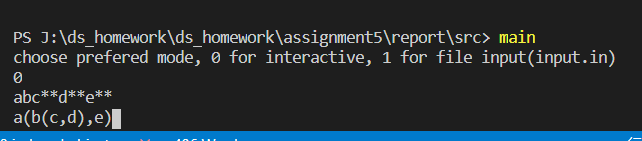
\includegraphics[width=0.5\textwidth]{images/样例1.png}
	\caption{样例}
\end{figure}
同时作为非法样例,还有a****
\begin{figure}[H]
	\centering
	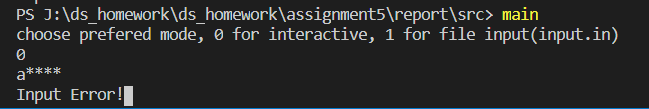
\includegraphics[width=0.5\textwidth]{images/样例2.png}
	\caption{非法样例}
\end{figure}